% !TeX spellcheck = de_DE
\chapter{Background}\label{background} 
This chapter gives a short introduction to topics regarding Agile processes and their definitions, Model Driven Architecture, Unified Modeling Language and Petri Nets. Basic knowledge in these topics helps us to appreciate the various design and implementation decisions taken in Chapter 3 and 4. This chapter also acts a guide to understand the various terminologies used throughout this work.

\section{Evolution of Agile Software Development}
Agile Software Development was introduced in the year 2001 by Agile Alliance to keep up with growing demands of the software industry. Traditional software development methods like Waterfall model couldn’t deliver the expected results on circumstances of frequent requirement changes and increased software complexity. The main reason that can be attributed to the failure of traditional development methods is the single flow of sequential development phases without any iterative phases.

For example, in Waterfall Model, the business analyst along with the client creates a set of requirements and a model of the final product. A requirement specification document is created which acts as the base document for the next development phases like Analysis, Design, Development and Testing of the product. The client is never involved during the development process and would view the product only after the final testing is completed. If the requirements of the client were not captured correctly or if the client has a changed requirement, then the entire development process has to be repeated. This kind of rework increases the cost, time and resources needed for the project and subsequently leads to its failure. (\cite{versionone}, \cite{getzephyr})

Agile Software Development, on the other hand, is built on the foundation of iterative approaches, in which product development happens incrementally and stakeholder participates in the entire \gls{sdlc} from the conception to the delivery of the product. One such methodology is \textit{Sprint} in which a larger functionality is broken into smaller pieces called \textit{User Stories} which can be delivered in a time span of just two weeks. This approach has several advantages such as the time consuming documentation is replaced with face to face communication with the stakeholders reducing the misinterpretation and hence a providing better understanding of stakeholder requirements.

Agile also provides separate methodologies for testing which makes testing easier with a quick feedback from stakeholders. A user story is marked complete if it passes all the acceptance tests. They are then evaluated whether to retain them for regression testing. A difference in interpretation of the requirement can be found out immediately with feedback and only a small rework will be needed in case of a difference. Test team members create the test plan, write test specifications and test cases and manage the testing activities within a sprint. The testing activities can be classified as follows.

\subsection{Requirements-Based Testing}
In this testing methodology, the objective is to verify whether the deliverable’s design and code meets the application’s requirements. Hence the test cases, conditions and data are generally derived from the requirements specification document. The testing can be done to verify either the functional attributes or the non-functional attributes like performance, reliability or usability. \cite{tahat2001requirement}

\subsection{Model-Based Testing}
This methodology involves the generation of test cases from models describing the system requirements and behavior. Even though this methodology requires the building of models up-front in the development cycle, it has several advantages like finding inconsistencies in the requirements itself and detection of discrepancies even before the code is generated. \cite{dias2007survey}

\subsection{Code-Based Testing}
In this methodology, test cases are used to evaluate the code to verify whether different test paths of the system are covered. The benefits of this methodology are that the parts of the software not tested in other techniques are covered. \cite{prasanna2005survey}

The main objective of this thesis is to simplify the existing test management process. As bulk of the effort is spent on elicitation and generation of test cases, this thesis aims to simplify the task of test case generation by using an automated tool. Most of the existing approaches for automated generation of test cases can be put under the above three categories. This thesis tries to automate test case generation for the first category which is Requirements-Based Testing.


\section{Model Driven Software Engineering}
An important paradigm shift happened in the field of software development after the introduction of \gls{mda} by \gls{omg}.   The underlying idea of \gls{mda} is to make use of models, a key tool in engineering, for software development. In general, models can be defined as abstraction of the system and its environment. An advantage with models is that it can be used to provide different levels of abstraction, with each level highlighting specific aspects or features of the system. Hence a model is essentially a representation of the necessary characteristics of the underlying system, leaving out the rest and thus contains less complexity. Less complexity of the models provides an easy way of system behavior prediction, examination of specific properties and unambiguous communication among software developers.

One of the motivations for \gls{mda} approach is that the developed software will be deployed to one or more platforms. The volatility of the platforms is higher than the higher-level models of the system and the objective of \gls{mda} is to create models that are increasingly independent of the target platform. In \gls{mda}, \glspl{pim} are initially designed in a platform independent language (e.g. \gls{uml}), which are then translated into \glspl{psm} by mapping them to some implementation language (e.g. C++, Java) as illustrated in Figure \ref{fig:Overview_MDA}.

\begin{figure}[htb!]
\centering
\fbox{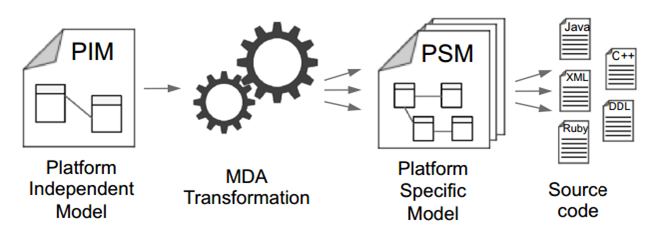
\includegraphics[width=0.8\textwidth]{content/images/Chapter2/Overview_MDA.png}}
\caption{Overview of transformations in MDA \cite{cerny2015separation}}
\label{fig:Overview_MDA}
\end{figure}

A number of \gls{omg} standards such as The \gls{uml}, \gls{xmi}, \gls{cwm}, \gls{mof} form the core of \gls{mda} concepts. Among these standards, \gls{uml} is used to define the \gls{pim} models which will be discussed in detail in the Section \ref{secuml} whereas the other standards are not in the scope of this thesis.

The term \gls{mdsd} or \gls{mdd} describes the family of engineering approaches that use models and their transformations for creating software products. \gls{mdsd} takes advantage of the \gls{mda} facilities, as a result of which the code can either be automatically or semi-automatically generated from models that are described in standard specification languages. The main priority of \gls{mdsd} is to enable the validation of software by the end users and customer stakeholders as early as possible in \gls{sdlc}.



\section{Unified Modeling Language} \label{secuml}
\gls{uml} is a standard from \gls{omg} and is a de-facto industry standard for modeling business applications using \gls{mdsd} \cite{cerny2015separation}. \gls{uml} models help to understand the requirements of the system graphically. They also provide aides to design the system, its components and to model the relationship existing between them right from early stages of software development. \gls{uml} also helps the developers and end users to maintain consistency in their interpretation of the design specification. \gls{uml}’s rapid gain in popularity in object oriented software development has attracted a great deal of research on \gls{uml} in software testing. (\cite{nebut2003requirements},\cite{badri2003use},\cite{nebut2003requirements})

\gls{uml} can be classified broadly into two categories namely structural and behavioral models. The structural diagrams represent the static structure of the system and the relationship between them. The different structural diagrams represent different abstraction and implementation levels. On the other hand, behavioral diagrams represent the dynamic behavior of the objects in the system i.e. the changes that happen in the system over time. Some of the important \gls{uml} diagrams which are used in upcoming sections are elaborated below.

Class Diagram is one example of structural diagrams that acts as a blueprint of the system or subsystem under development. It is extensively used to model the objects that make up the system, the relationship between them, their description and the functions they provide. Class Diagrams usage is across different levels in the development cycle. In analysis stage, it is used to understand the requirements of the problem domain whereas, in the implementation stage, it can be used to create actual software classes. An example of Class Diagram is shown in Figure \ref{fig:umldiagrams_subfigA}.

Activity Diagram is one example of behavioral diagrams which illustrates the sequence of actions in a process. Activity Diagrams usage across different levels in the development cycle are illustrated below. In requirements stage, it can be used to model the flow of events that the use cases describe and in design and implementation stage, it can be used to define the behavior of operations. An example of Activity Diagram is shown in Figure \ref{fig:umldiagrams_subfigB}.

\begin{figure}[htb!]
  \centering
    \subfloat[]{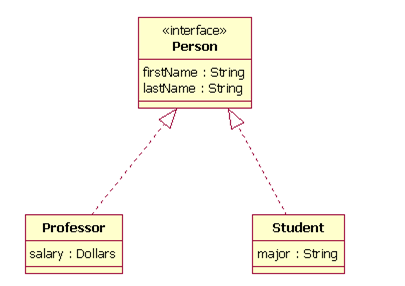
\includegraphics[width=0.4\textwidth,frame]{content/images/Chapter2/ClassDiagram.png} \label{fig:umldiagrams_subfigA}}
   \subfloat[]{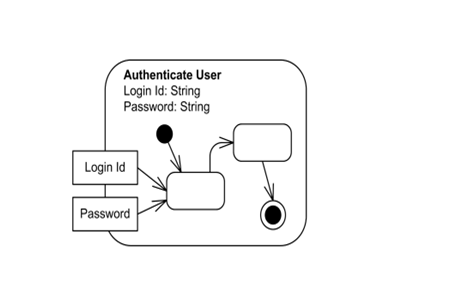
\includegraphics[width=0.4\textwidth,frame]{content/images/Chapter2/ActivityDiagram.png} \label{fig:umldiagrams_subfigB}}
	\caption{An example of a) UML Class Diagram for personal details b) UML Activity Diagram for user authentication.}
\label{fig:umldiagrams}
\end{figure}

\section{Petri Net}
Petri Net is a graphical and mathematical modeling tool with well defined semantics suitable for formal analysis. The concept of Petri Net was first introduced by Carl Adam Petri in the year 1961, after which it had grown tremendously to support different domains like workflow management, manufacturing, real time systems, distributed systems, embedded systems, protocols and networks, performance evaluation and much more.
 
In the domain of computer science engineering, Petri nets are mainly used in information processing systems that can be categorized as parallel, concurrent, distributed, asynchronous, non-deterministic and stochastic. Petri nets can be used as communication documents like flow charts, block diagrams and networks but can also simulate the dynamic and concurrent activities of the system with the concept of tokens. Also, it can model the mathematical representations of the systems using algebraic and state equations. 

\subsection{Basics of Petri Net}
There are different kinds of Petri Nets depending upon the amount of information that the nets can carry. One such example of low level Petri Net is the Place/Transition Net (PT-Net) which is used in this thesis.

A Petri Net is an example of directed, bipartite and weighted graph in between two nodes called places and transitions. Arcs run between places and transitions and each place can hold specific items called tokens. An example Petri Net is shown in Figure \ref{fig:petrinet_example} and the various elements are elaborated below.

\begin{figure}[htb!]
\centering
\fbox{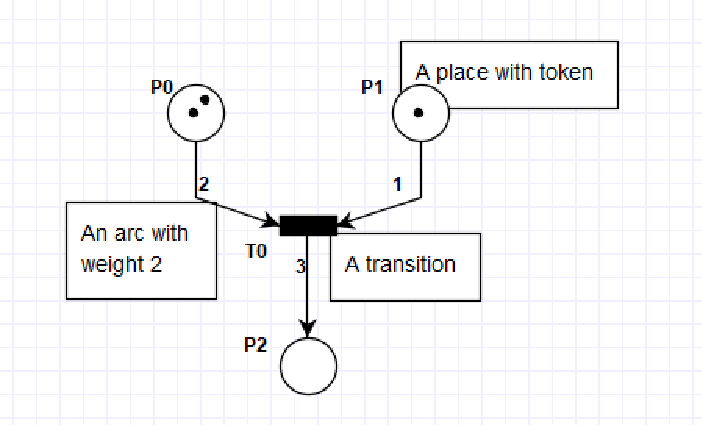
\includegraphics[width=0.5\textwidth]{content/images/Chapter2/Petrinetwithlabels.png}}
\caption{An example of a Petri Net}
\label{fig:petrinet_example}
\end{figure}

\textbf{\textit{Places}} are the passive component of the net, and they represent the buffer, communication medium or in general a geographical location. The current state of the system is determined by the number of tokens present in a place and this state is represented by the term \textit{Marking} in Petri Nets.

\textbf{\textit{Transitions}} are the active components of the net, which represent the activities that change the state of the system. Transitions are fired only when certain preconditions are met and these conditions are represented in the net by means of tokens.

\textbf{\textit{Tokens}} are present inside the places and each token represents a condition to be fulfilled or a synchronization condition. In general, tokens represent a physical or information object.

\textbf{\textit{Arcs}} run only between places and transitions or vice versa. In the first case, these are called \textit{input arcs} whereas in the second case these are called \textit{output arcs}. Each arc is also associated with a specific weight that determines the number of tokens required for firing the particular transition.

\subsection{Formal Definition and Basic Terminology}
The terms defined in the above section can be formally defined as the following. The definitions are an excerpt from Calisaya et. al., 2015 \cite{calisaya2016analysis}.

\begin{definition}
\label{def:def1}
A \textbf{place-transition Petri Net} \cite{reisig2012petri}  is a five-tuple PN = (P, T, F, W, M$_{0}$) where P = $ \lbrace $p$_{1}$, p$_{2}$, ..., p$_{n} \rbrace $ is a finite set of places, T = $ \lbrace $t$_{1}$, t$_{2}$,..., t$_{n} \rbrace $ is a set of transitions, F   (P $\times$ T) $ \cup $ (T $\times$ P) is a set of arcs, W : F $ \subseteq $ $ \rightarrow$ $ \lbrace $1, 2,...$ \rbrace $ is a weight function, M$_{0}$ : P  $ \rightarrow\lbrace $0, 1, 2, ...$ \rbrace $ is the initial marking and P $ \cap $ T = $\emptyset $ and P $ \cup $ T 
$ \neq $ $ \emptyset $.
\end{definition}

\begin{definition}
\label{def:def2}
For a PN = (P, T, F, W, M$_{0}$), a \textbf{marking} is a function M: P $  \rightarrow$ $ \lbrace $0, 1, 2,...$ \rbrace $, where M (p) is the number of tokens in p. M$_{0}$ represents the initial marking of PN.
\end{definition}


\begin{definition}
\label{def:def3}
A \textbf{transition} t is enabled for firing at a marking M if M (p) $ \geq $ W (p, t) for any p $ \in $ p$ _{in} $ where p$ _{in} $ is the set of input places of t. On firing t, M is changed to M' such that $ \forall $p $ \in $ P: M' (p) = M (p) - W (p,t) + W (t,p). 
\end{definition}

\begin{definition}
\label{def:def4}
For a PN, a sequence of transitions $ \sigma $ = $ \langle $t$_{1}$, t$_{2}$, ..., t$_{n} \rangle $ is called a \textbf{firing sequence} if and only if M$_{0}$[t$_{1} \rangle $, [t$_{2} \rangle $,..., [t$_{n} \rangle $M$_{n}$. In notation, M$_{0}$ [PN, $ \sigma \rangle $M$_{n}$ or M$_{0}$ [$ \sigma \rangle $M$_{n}$.
\end{definition}

\begin{definition}
\label{def:def5}
For a PN = (P, T, F, W, M$_{0}$), a marking M is said to be \textbf{reachable} if and only if there exist a firing sequence $ \sigma $ such that M$_{0}$ [$ \sigma \rangle $M.
\end{definition}


\subsection{Analysis of Petri Nets}
One of the main features of Petri Net is the ability to perform analysis on model properties i.e. it can detect defects related to structural and dynamic properties \cite{murata1989petri}. A simple transversal of the flow relation between places and transitions can detect the structural properties whereas initial markings and final markings after transitions can detect the dynamic properties. As defined in \cite{reisig2012petri}, the defects due to dynamic properties of boundedness, liveliness, deadlock free and reachability can be detected using methods like simulation, reachability/coverability or invariant analysis.

 The transition behavior in a Petri Net is shown in Figure \ref{fig:petridiagrams}. Figure \ref{fig:petridiagrams} (a \& b) show Petri Nets with markings M0 and M1 respectively.  P0 and P1 are the places and T0 is the transition. The places contain tokens and arcs with arc weight of two and one respectively. This marking, which is the required precondition, enables the firing of the transition T0 and subsequently results in the marking as shown in Figure  \ref{fig:petrinet_subfigB}.  The final marking consists of place P2 with three tokens since the arc from T0 to P2 is of weight 3. 

\begin{figure}[htb!]
  \centering
    \subfloat[before transition]{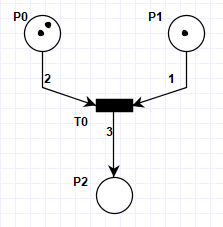
\includegraphics[width=0.3\textwidth,frame]{content/images/Chapter2/Petrineta.png} \label{fig:petrinet_subfigA}}
   \subfloat[after transition]{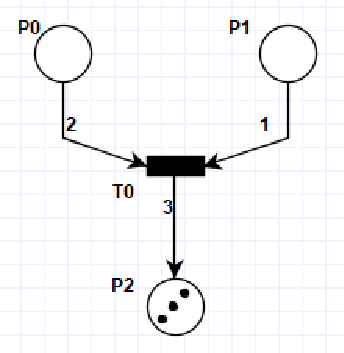
\includegraphics[width=0.3\textwidth,frame]{content/images/Chapter2/Petrinetb.png} \label{fig:petrinet_subfigB}}
	\caption{Concept of transition in a Petri Net.}
\label{fig:petridiagrams}
\end{figure}


